
\section{Conservation of Angular Momentum}

\instructornote{%
This lab was significantly rewritten in Fall 2021 by Matt Trawick.

Rather than using Tracker to take a movie (which is pretty slow), the lab now uses Capstone and a photogate to measure the angular velocity $\omega$ of the disk.  

Also, I've discovered that putting masking tape around the disk keeps the mass from falling off, and also virtually guarantees that the final position of the weight will be right up against the edge of the disk, allowing moment of inertia $I_{\rm final}$ to be calculated ahead of time.  This trick with the masking tape is easily the second smartest thing I've ever done in my life, right after figuring out that ``el-em-en-oh'' in the alphabet song is actually four different letters.

Finally, I rewrote the error analysis part.  Previous version asked students to go around the classroom asking everybody else for their initial and final angular momenta, and then make a histogram of the differences to look for systematic error.  In this version I ask students to estimate the uncertainty in the angular velocity, and then (presumably) use that to estimate the uncertainty of the angular momentum.

This lab has gone back on forth on whether to instruct students to use the parallel axis theorem to calculate the moment of inertia of the dropped mass.  (Treating it as a point mass instead introduces an error of about 3\% in the moment of inertia of the weight.)  In this version, I tell students to use the parallel axis theorem if they know how.

Additional question: You can ask students to calculate the initial and final mechanical energy of the system, and ask
them whether mechanical energy was conserved.  They are often surprised to discover that it's not.  Then you can ask them what external force is responsible for the work apparently done on the system, and they generally get stumped.  (They don't get that there's friction as the mass slides.)
}

\makelabheader %(Space for student name, etc., defined in master.tex or labmanual_formatting_commands.tex)

%\textbf{Objectives} 
%
%To test the Law of Conservation of Angular Momentum and to explore the applicability
%of angular momentum conservation among objects that experience no external torques. 

\begin{wrapfigure}[4]{r}{0.35\textwidth}
%    \vspace{-0.3in}
    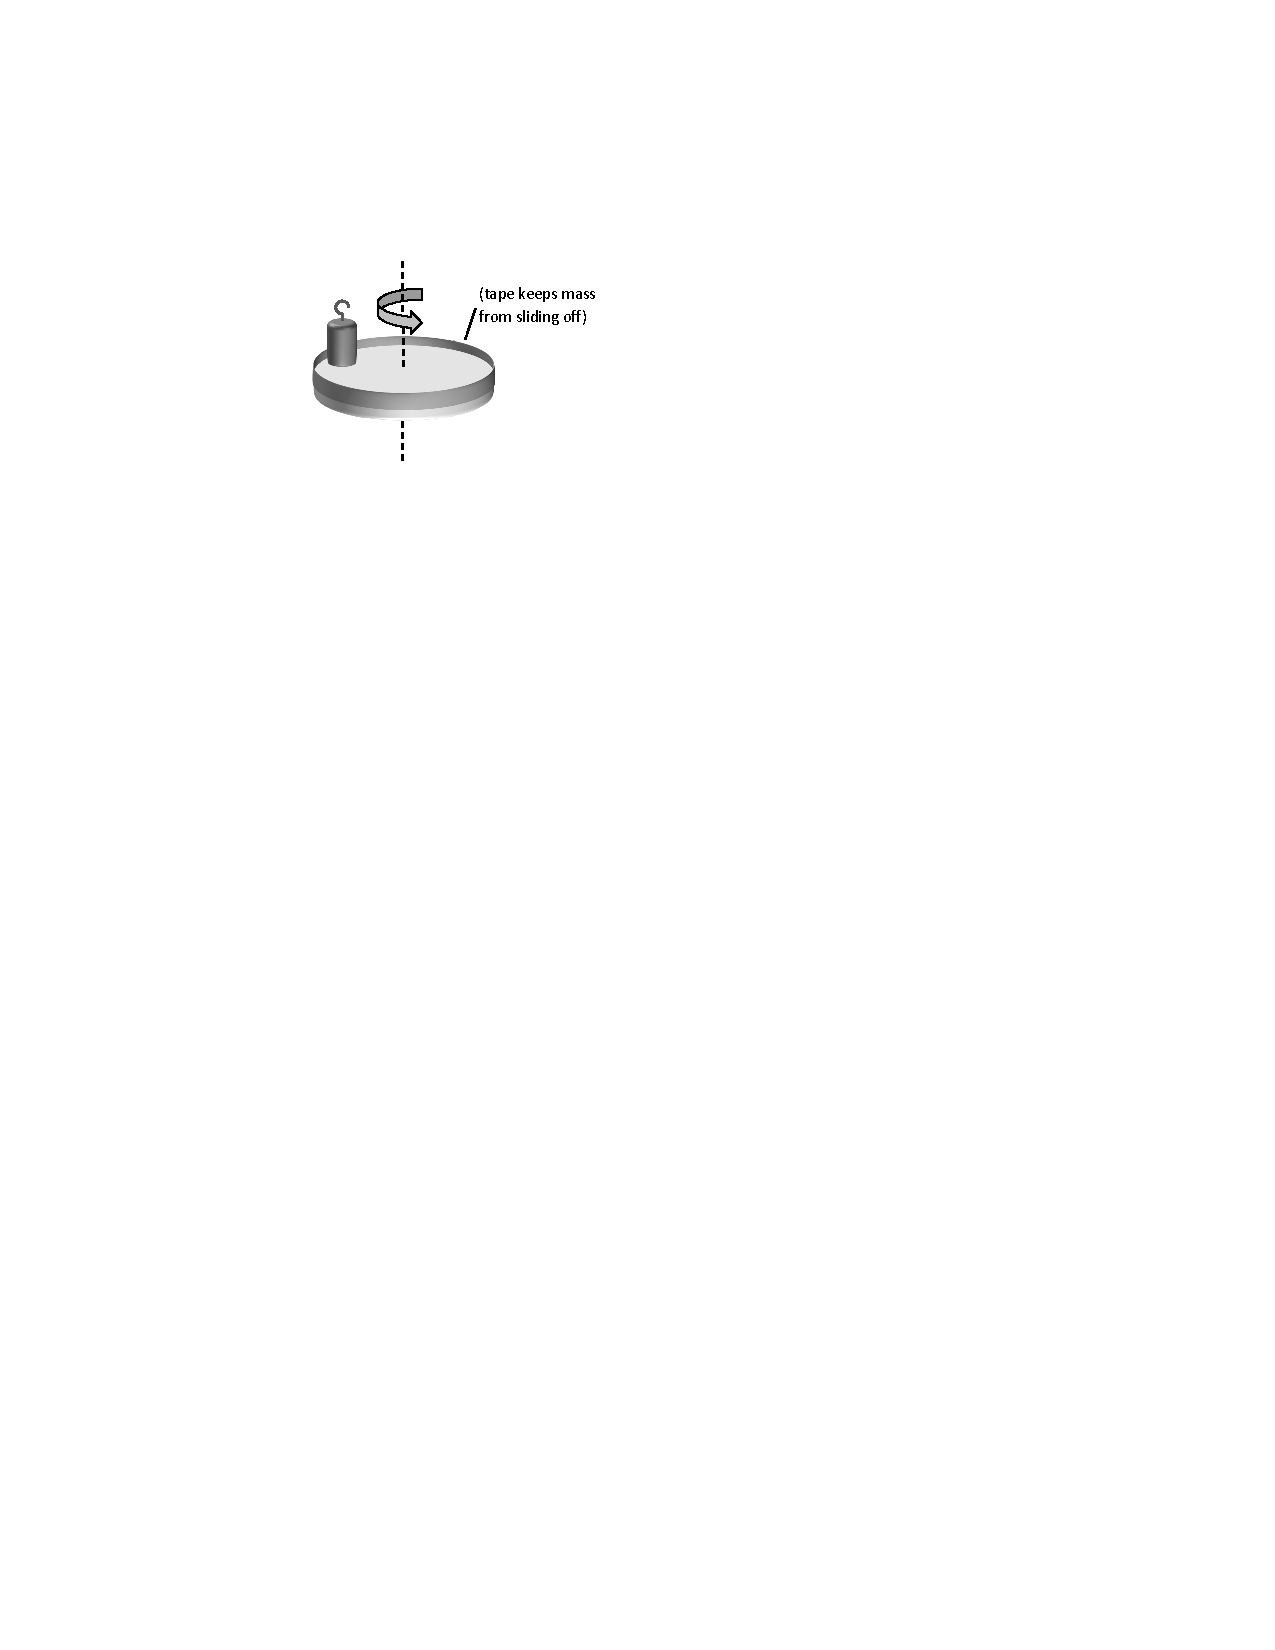
\includegraphics{cons_ang_mom/apparatus_fig.pdf}
\end{wrapfigure}

\bigskip

\textbf{Apparatus}

\begin{itemize}[nosep]
\item Rotating disk system, with paper tabs 
\item Photogate and Pasco interface
\item Masses of 500 g, 1 kg 
\item Simple cm ruler 
\item Vernier caliper
\item Small water bubble level
%\item A video analysis system (\textit{Tracker})
\item \textit{Capstone} software (\filename{conserve\_ang\_mom.cap} experiment file)
\item Masking tape
\end{itemize}

\bigskip
\textbf{Overview }

As a consequence of Newton's laws, angular momentum like linear momentum is
believed to be conserved in isolated systems. This means that, no matter how
many internal interactions occur, the total angular momentum of any system should remain constant if there are no external torques. When one of the objects gains some angular momentum another part of the system must lose the same amount. If angular momentum isn't conserved, then we believe that there is some outside torque acting on the system. 

In this unit you will test the notion of the conservation of angular momentum.
As in the test of the conservation of linear momentum, we will investigate what
happens when two bodies undergo a ``rotational'' collision.
You will drop a large weight onto a rotating disk and determine 
%the moment of inertia, the angular speed, and finally, 
the angular momentum of the rotator-disk-weight
system before and after this perfectly inelastic collision.

\medskip
\textbf{Activity 1: The Moment of Inertia Before and After the Collision}

(a) Calculate the theoretical value of the moment of inertia of the disk
using basic measurements of its radius and mass. Be sure to include units and
show the expression you used!
\vspace{5mm}

\hspace{0.5in}\( R_{d} =\)  \hfill{}\( M_{d}= \) \hfill{}
\vspace{5mm}

\hspace{0.5in}\( I_{d}= \)
\vspace{5mm}

After dropping the weight on the rotating disk, the system will have a new
moment of inertia. 

(b) First, record the mass $m_w$ and radius $r_w$ of the weight, as well as the distance $d$
that the center of weight will be from the center of the disk once it slides all the way to the
masking tape.  You can use the vernier calipers to measure the weight's diameter.

\medskip
\hspace{0.5in}$m_w=$ \hfill $r_w=$ \hfill $d=$ \hfill 
\bigskip

(c) Next, write down a formula for the moment of inertia $I_w$ of the weight as it revolves with the disk, 
and calculate its value based on your measurements above.  
(If you know how to use the parallel axis theorem, use it!  If not, you can treat the weight as just
a point mass a distance $d$ from the center of the disk, which turns out to be a reasonable approximation here.)

\medskip
\hspace{0.5in} $I_w =$
\answerspace{0.6in}
\pagebreak[3]

%(You can treat the weight like a point particle.\footnote{Of course the weight isn't 
%(actually a point particle.  For a really precise calculation, you would also need 
%(to account for its shape and its rotation about its own center of mass, 
%(using the \textit{parallel axis theorem}.}  

(c) What is the moment of inertia $I_{\rm final}$ of the whole system after the mass has been dropped on the disk?

\medskip

\hspace{0.5in} $I_{\rm final}$ = 
\answerspace{0.4in}

\bigskip
\textbf{Activity 2: Measurement of Angular Velocity and Angular Momentum}

Open the experiment file \filename{conserve\_ang\_mom.cap} in the \filename{\coursefolder} folder.  
You will be using a photogate to measure the angular speed $\omega$ of the rotating disk.  The photogate simply measures the elapsed time whenever its beam is broken.  The experiment file has already been set up to calculate $\omega$ from these measured times.  (You're welcome!)

Set up your photogate so that its beam is periodically broken by the paper sticking out from between the disks.  When you are ready, give the disk a moderate spin, and hit record in the program.  Wait a few seconds to get a stable measurment of the initial angular speed, then drop the weight gently on the spinning disk, continuing to record the speed for a few seconds.  Print out your graph of $\omega$ vs. time if your instructor requests it.

(a) From your graph, determine the angular speeds $\omega_{\rm initial}$ and $\omega_{\rm final}$ of the system both before and after the collision.  Note that there's probably a little bit of friction in the system, which means the speed won't ever be exactly constant.  You'll need to think about how to handle this, and use this to estimate and record the uncertainty $\pm \delta \omega$ for each of your measurements.

\medskip
\hspace{0.5in} $\omega_{\rm initial} =$

\bigskip
\hspace{0.5in} $\omega_{\rm final} =$
\answerspace{0.3in}

(b) How did you estimate your uncertainties $\pm \delta \omega$, above?
\answerspace{1 in}

(c) Calculate the angular momentum $L$ before and after the collision (including units!).  Be sure to include the uncertainty $\pm\delta L$ for each.

\medskip
\hspace{0.5in} $L_{\rm initial} =$
\answerspace{0.6in}

\hspace{0.5in} $L_{\rm final} =$
\answerspace{0.6in}

(d) Was the angular momentum of the system conserved during this collision, to within the precision of your measurement?  If not, can you think of any reasons why it might not have been?
\answerspace{0.6in}


